\section{Single phase consolidation}
Let us begin by introducing a few governing equations.

\subsubsection*{Fluid mass and momentum balance}
Linear momentum balance for the fluid follows Darcy:

\begin{equation}
{v}_{ri}=\phi \left( {{v}_{i}}-{{v}_{si}} \right)=-\frac{{{k}_{ij}}}{\mu }\left( \frac{\partial p}{\partial {{x}_{j}}}+\rho {{g}_{j}} \right),
\label{eqch14:genmass}
\end{equation}

for the intrinsic permeability, ${{k}_{ij}}$, dynamic viscosity, $\mu $, and density, $\rho $. The subscript $r$ considers that fluid velocity is relative to motion of the deformable solid (${{v}_{si}}$), so that ${{v}_{i}}$ is absolute fluid velocity, and ${{v}_{ri}}$ is relative. Conservation of fluid mass requires,

\begin{equation}
\frac{\partial }{\partial t}\left( \phi \rho  \right)+\frac{\partial }{\partial {{x}_{i}}}\left( \phi \rho {{v}_{i}} \right)=0.
\end{equation}
	
Fluid properties are functions of temperature and pressure. The fluid density time derivative appearing in the mass balance equation may be expanded to

\begin{equation}
\frac{d\rho}{dt}=\rho \left( \frac{1}{K_{f}^{p}}\frac{dp}{dt}-\frac{1}{K_{f}^{T}}\frac{dT}{dt} \right),
\end{equation}
	
with fluid compressibility given by $1/K_{f}^{p}={{\left. \left( 1/\rho  \right)\left( \partial \rho /\partial p \right) \right|}_{T}}$ and for the fluid thermal expansion coefficient $1/K_{f}^{T}=-{{\left. \left( 1/\rho  \right)\left( \partial \rho /\partial T \right) \right|}_{p}}$. In these definitions we utilize moduli ($K$ = inverse compressibility). Also, because thermal effects are not considered in these examples, the temperature dependence may be neglected. Utilizing the Lagrangian total derivative of a component relative to the moving solid, ${{d}_{s}}/dt=\partial /\partial t+{{v}_{si}}\partial /\partial {{x}_{i}}$, and a moving fluid, ${{d}_{f}}/dt=\partial /\partial t+{{v}_{fi}}\partial /\partial {{x}_{i}}$, substituting for absolute fluid velocity and dividing through by density gives,

\begin{equation}
\phi \left( \frac{1}{K_{f}^{p}}\frac{dp}{dt}+\frac{{{d}_{s}}\phi }{dt}+\frac{\partial {{v}_{si}}}{\partial {{x}_{i}}} \right)=-\frac{\partial }{\partial {{x}_{i}}}\left( {{v}_{ri}} \right).
\end{equation}
	
To obtain the porosity time derivative, we expand the solid mass balance to obtain

\begin{equation}
\frac{{{d}_{s}}\phi }{dt}=\frac{\left( 1-\phi  \right)}{{{\rho }_{s}}}\frac{\partial {{\rho }_{s}}}{\partial t}+\left( 1-\phi  \right)\frac{\partial {{v}_{si}}}{\partial {{x}_{i}}}.
\end{equation}
	
Substituting this gives,

\begin{equation}
\frac{\phi }{K_{f}^{p}}\frac{dp}{dt}+\left[ \frac{\partial {{v}_{si}}}{\partial {{x}_{i}}}+\frac{\left( 1-{{\rho }_{s}} \right)}{{{\rho }_{s}}}\frac{\partial {{\rho }_{s}}}{\partial t} \right]=-\frac{\partial }{\partial {{x}_{i}}}\left( {{v}_{ri}} \right).
\end{equation}
	
Utilizing Biot's formulation to represent the solid density time derivative and assuming small strain yields the full fluid mass balance (\cite{KhaliliSelvadurai:03} and \cite{RutEtAl:01}),

\begin{equation}
\left( \frac{\phi }{K_{f}^{p}}+\overbrace{\frac{\left( \alpha -\phi  \right)}{{{K}_{g}}}}^{A} \right)\frac{dp}{dt}+\overbrace{\alpha \frac{\partial {{v}_{si}}}{\partial {{x}_{i}}}}^{B}=-\frac{\partial }{\partial {{x}_{i}}}\left( {{v}_{ri}} \right),
\label{eqch14:flmass}
\end{equation}
	
where ${{K}_{g}}$ is the solid grain bulk modulus, and $\alpha$ is the Biot-Willis coefficient ($\alpha =1-K/{{K}_{g}}$ in an ideal, fully interconnected porous media). The bracketed terms $A$ and $B$ represent important couplings from the mechanical system to that of the fluid. All are vital in the HM procedure and without them the equation simplifies to a standard fluid flow equation with fluid compressibility storage in the pressure time derivative. 

\subsubsection*{Solid momentum balance}

We begin with the concept of effective stress,

\begin{equation}
\sigma {{'}_{ij}}={{\sigma }_{ij}}+\alpha p{{\delta }_{ij}},
\end{equation}

for the effective stress, $\sigma '$, and the total stress, $\sigma$; negative in compression. Balance of linear momentum is defined by,

\begin{equation}
\frac{\partial {{\sigma }_{ij}}}{\partial {{x}_{j}}}+{{F}_{i}}=0,
\end{equation}

for the body force, $F=\rho _m \text{g}$ and where $\rho _m =\phi \rho _f + (1-\phi )\rho _s$ is density of the mixture. From the definition of strain, ${{\varepsilon }_{ij}}=\left( \partial {{u}_{i}}/\partial {{x}_{j}}+\partial {{u}_{j}}/\partial {{x}_{i}} \right)/2$, and an arbitrary stress-strain relationship of the form $\mathbf{\sigma }=\mathbf{D\varepsilon }\left( \mathbf{u} \right)$, we write the displacement formulation of mechanical equilibrium (neglecting thermal effects) for isotropic linear elasticity,

\begin{equation}
\frac{\partial }{\partial {{x}_{j}}}\left[ G\frac{\partial {{u}_{i}}}{\partial {{x}_{j}}}+\left( \lambda +G \right)\frac{\partial {{u}_{j}}}{\partial {{x}_{i}}}-\alpha p{{\delta }_{ij}} \right]+{{F}_{i}}=0,
\label{eqch14:mequil}
\end{equation}

where $G$ and $\lambda$ are the Lam� constants. Changes to the fluid system are therefore visited in mechanical equilibrium via the effective stress.

\subsubsection*{Numerical solution scheme}
The numerical solution of Eqs. \ref{eqch14:flmass} and \ref{eqch14:mequil} can be obtained with any convenient method. In these benchmarks, we use a standard Galerkin finite element spatial discretization with time discretization following a generalized first order finite difference scheme, as implemented in OpenGeoSys. Note that Eq. \ref{eqch14:mequil} is an equilibrium equation, and has no time dependency other than that imposed by coupling terms to fluid behavior. The result is a set of coupled linear equations in pressure, $p$, and solid displacement, $u$. The two equations may be solved sequentially and iteratively, or monolithically as a single system. We present results using both solution schemes in the following benchmarks.

%-------------------------------------------------------------------------
%-------------------------------------------------------------------------

\subsection{Terzaghi consolidation: Monolithic and staggered approaches}

In the HM problem, mechanical compression generates a fluid pressure response, while pressure storage and dissipation affect the mechanical condition via the effective stress. Terzaghi has provided the framework to test such a problem. A cartoon of the problem to be examined is shown in Fig. \ref{terz:cartoon}. This test is a necessary, but not fully sufficient condition for correct implementation of a hydromechanical simulator. It guarantees correct implementation of the coupling relationships between the 1)fluid and 2)mechanical system.

\begin{figure}[!tbh]
\begin{center}
\includegraphics[width=0.7\textwidth]{chapter_14/figures/fig_14_1_1}
\end{center}
\caption{Terzaghi problem. A.) 2-D column ($p=0$ initially) stress applied to top of column which is a free draining boundary. Other boundaries are no-flow and roller displacement. Stress may be applied as a single step-load, or as a function of time. Pressure and displacement are monitored in time at specific locations. B.) Anticipated (conceptual) pressure profiles within the column with the progression of time for a step-load of applied stress (in full column, not at monitoring locations).}
\label{terz:cartoon}
\end{figure}

\subsubsection*{Definition}
For a single fluid phase, the analytical solution for pressure dissipation is available.  The analytical solution to this problem has been utilized a number of times for this very purpose. Beginning from the 1-D fluid diffusion equation of hydrogeology (simply a fluid mass balance equation),

\begin{equation}
\frac{\partial p}{\partial t}-c\frac{{{\partial }^{2}}p}{\partial {{z}^{2}}}=0,
\end{equation}

where $c$ is 1-D fluid diffusivity.  The pore pressure response to a vertical load, $\sigma _{z}$, applied linearly over time ($\sigma _{z}^{t={{0}^{-}}}=0$) to the top of the column at a rate, ${{\dot{\sigma }}_{z}}=d{{\sigma }_{z}}/dt$, is, (\cite{Wang:00}, Eq. 6.50),

\begin{equation}
\begin{split}
\frac{p\left( z,t \right)}{{{p}_{0}}}=\left\{ 1-{{\left( \frac{L-z}{L} \right)}^{2}}-\right.\left. \frac{32}{{{\pi }^{3}}}\left[ \sum\limits_{m=0}^{\infty }{\frac{{{\left( -1 \right)}^{m}}}{{{\left( 2m+1 \right)}^{3}}}\exp \left[ -{{\psi }^{2}}ct \right]\cos \left[ \psi \left( L-z \right) \right]} \right] \right\},
\end{split}
\end{equation}

where the total pressure generation is

\begin{equation}
{{p}_{0}}=\frac{{{L}^{2}}}{2c}\left( {{B}_{v}}{{{\dot{\sigma }}}_{z}} \right),
\end{equation}

for the factor, $\psi =\left( 2m+1 \right)\pi /\left( 2L \right)$, the total column length, $L$, and the location in the column (downward from the applied stress), $z$. The 1-D Skempton coefficient,

\begin{equation}
{{B}_{v}}={{\left. -\frac{\delta \bar{p}}{\delta {{\sigma }_{zz}}} \right|}_{{{\varepsilon }_{xx}}={{\varepsilon }_{yy}}=\zeta =0}}=\frac{\alpha }{{{K}_{v}}{{S}_{v}}},
\end{equation}

is given purely by micromechanical, poroelastic considerations from the uniaxial drained bulk modulus, $K_{v}$, and the 1-D specific storage, $S_{v}$ (Table \ref{terz:tab1}). The 1-D diffusivity is also a derivative of the 1-D storage:

\begin{equation}
c=\frac{k}{\mu {{S}_{v}}},
\end{equation}

and also the permeability, $k$, and viscosity, $\mu$. See Table \ref{terz:tab1}, \cite{DetournayCheng:93}, and \cite{Wang:00} for additional details regarding poroelastic relationships. If utilizing an applied step load at time $t={{0}^{+}}$ we can generate another analytical solution for pressure, and also displacement. For this validation, we utilize only the linear loading rate. Because displacement is the primary variable in our FEM formulation, the displacement must be accurate in order to generate the correct pressure response: we find no need to reproduce the results of a step load analysis here.

\begin{table}[!htb]
\begin{center}
\begin{tabular}{lll}
\hline\noalign{\smallskip}
Parameter & Description & Equation \\
\noalign{\smallskip}\hline\noalign{\smallskip}
$B$         & Skempton coefficient & ${\alpha }/{\left[ \alpha -\phi \left( 1-\alpha  \right)+\phi K/{{K}_{f}} \right]}\;$ \\
$K^{u}$     & Undrained bulk modulus & $K/\left( 1-\alpha B \right)$ \\
$G$         & Shear modulus & $3K\left( 1-2\nu  \right)/\left( 2+2\nu  \right)$ \\
$\nu ^{u}$  & Undrained Poisson's ratio &  ${\left( 3{{K}^{u}}-2G \right)}/{\left( 6{{K}^{u}}+2G \right)}\;$ \\
$B_{v}$     & Uniaxial Skempton coefficient &  $B{\left( 1+{{\nu }_{u}} \right)}/{\left( 3-3{{\nu }_{u}} \right)}\;$ \\
$K_{v}$     & Uniaxial bulk modulus & $3K{\left( 1-\nu  \right)}/{\left( 1+\nu  \right)}\;$ \\
$K_{v}^{u}$ & Uniaxial undrained bulk modulus & ${3{{K}^{u}}\left( 1-{{\nu }^{u}} \right)}/{\left( 1+{{\nu }^{u}} \right)}\;$ \\
$S_{v}$     & Uniaxial storage & ${\alpha }/{\left( {{K}_{v}}{{B}_{v}} \right)}\;$ \\
\noalign{\smallskip}\hline
\end{tabular}
\end{center}
\caption{Fundamental poroelastic relationships. Many potential combinations are available, these representing only one possibility.}
\label{terz:tab1}
\end{table}

We choose a rather long (50m) column of rock with material properties similar to those of Berea sandstone (Table \ref{terz:tab2}).  The column is discretized uniformly into 50 FEM grid cells. Geometry is shown in Fig. \ref{terz:cartoon}, which shows a single column surrounding by displacement roller boundaries allowed to compress from the top where a loading rate, ${{\dot{\sigma }}_{z}}$, is applied at time $t=0^{+}$. Fluid pressure is initially null. Compression of the column leads to a rapid pressure increase and a subsequent drainage of pressure over time from the top of the column. The load is applied quickly enough to allow pressure to build with time. The topmost boundary is free drainage for fluid flow, all others being no-flow.

\begin{table}[!htb]
\begin{center}
\begin{tabular}{lccl}
\hline\noalign{\smallskip}
Property & Symbol & Unit & Value \\
\noalign{\smallskip}\hline\noalign{\smallskip}
\textit{Berea sandstone} & & & \\
Drained bulk modulus & $K$ & $GPa$ & 8.0 \\
Poisson ratio & $\nu $ & $-$ & 0.20 \\
Porosity & $\phi $ & $-$ & 0.19 \\
Permeability & $k$ & $m^{2}$ & $1.9\times 10^{-13}$ \\
Biot-Willis coefficient & $\alpha $ & $-$ & 0.8 \\
 & & & \\
\textit{Westerly granite} & & & \\
Drained bulk modulus & $K$ & $GPa$ & 25.0 \\
Poisson ratio & $\nu $ & $-$ & 0.25 \\
Porosity & $\phi $ & $-$ & 0.02 \\
Permeability & $k$ & $m^{2}$ & $5.0\times 10^{-15}$ \\
Biot-Willis coefficient & $\alpha $ & $-$ & 0.6 \\
\noalign{\smallskip}\hline
\end{tabular}
\end{center}
\caption{Solid properties.}
\label{terz:tab2}
\end{table}

\begin{table}[!htb]
\begin{center}
\begin{tabular}{lccc}
\hline\noalign{\smallskip}
Property & Symbol & Unit & Value \\
\noalign{\smallskip}\hline\noalign{\smallskip}
Bulk modulus   & $K_{f}$      & $GPa$         & $2.27$ \\
Density        & $\rho $      & $kg/m^3$      & $997.05$ \\
Viscosity      & $\mu $       & $Pa\times s$    & $8.9008\times 10^{-4}$ \\
\noalign{\smallskip}\hline
\end{tabular}
\end{center}
\caption{Fluid properties.}
\label{terz:tab3}
\end{table}

\subsubsection*{Results}

Simulations are conducted using both a staggered (fluid and solid equations solved iteratively) and monolithic (fluid and solid equations solved in a single matrix) with OpenGeoSys. Results are shown in Fig. \ref{terz:res1} for two alternate material property scenarios: Berea sandstone and Westerly granite. The solution is accurate in all cases. We note a small inaccuracy in the slower loading rate for sandstone that illustrates the impact of tolerance in the time step control. Here, we add one extra data set (small dots) with tighter time control, which shows that tighter accuracy can be achieved with this adjustment.

\begin{figure}[!tbh]
\begin{center}
\includegraphics[width=1.0\textwidth]{chapter_14/figures/fig_14_1_2}
\end{center}
\caption{Results of HM coupling.}
\label{terz:res1}
\end{figure}

While the monolithic solution is unconditionally stable for an implicit time-stepping scheme, the staggered solution suffers limitations. When the fluid becomes highly incompressible relative to the solid, the solution will diverge. We provide the general criterion that stability is achieved with $B_v<0.5$. This criterion is generally independent of loading rate. The implications of this are important, such that for Westerly granite if incompressible grains are used the solution is unstable at $25 ^{o}C$ for the properties of Table \ref{terz:tab2}. Stability can be enforced by increasing the value of porosity that is used, or decreasing $\alpha $, or with any adjustment that brings $B_v$ above 0.5. The staggered solution is stable for all realistic cases (everything compressible) we have tried. For very sharply applied loads such as a step load applied at $t=0^+$, however, the staggered solution will become unstable even with this criterion. It is important for a given problem and set of solid/fluid properties to examine stability with the above benchmark before extending to the full system.

Time steps are adaptively controlled with a tolerance based on the rate of pressure change over a time step. Such a scheme is capable of ensuring accuracy in HM or H$^2$M problems. Note the importance of the tolerance in Fig. \ref{terz:res1}.
\subsection{Distributed footing: Poroelastic cube (3D)}
We consider a vertical cross-section through homogeneous soil. Due to symmetry we can limit the investigation to half of the domain. The model domain is then extending 8 meters in length and 5 meters in height. The problem is solved in 2D and 3D space, respectively.

\begin{figure}[!tbh]
\begin{center}
\scalebox{1.0} % Change this value to rescale the drawing.
{
\begin{picture}(380,190)
\put(70,160){\line(1,0){240}}
\put(310,10){\line(0,1){150}}
\multiput(70,10)(0,11){14}{\line(0,1){7}}
\put(75,180){\vector(0,-1){20}}
\put(80,180){\vector(0,-1){20}}
\put(85,180){\vector(0,-1){20}}
\put(90,180){\vector(0,-1){20}}
\put(95,180){\vector(0,-1){20}}
\put(308,165){8}
\put(60,165){0}
\put(55,8){-5}
% BC
% left
\put(5,100){$\frac{\partial p}{\partial x} = 0$}
\put(5,85) {$u_x = 0$}
\put(5,75) {$\sigma_{xy} = 0$}
% top
\put(75,150){$\sigma_{yy}=\sigma_0$}
\put(75,140){$\sigma_{xy}=0$}
\put(180,165){$\sigma_{xy}=\sigma_{yy}=0$}
\put(210,187){\vector(1,0){100}}
\put(175,187){\vector(-1,0){105}}
\put(180,185){$p=0$}
% right
\put(320,100){$\frac{\partial p}{\partial x} = 0$}
\put(320,85) {$u_x = 0$}
\put(320,75) {$\sigma_{xy} = 0$}
% bottom
\put(160,-5){$\frac{\partial p}{\partial y} = 0$ , $u_x=u_y=0$}
\linethickness{2pt}
\put(70,10){\line(1,0){240}}
\end{picture}
}
\end{center}
\caption{Conceptualization of the footing problem. Properties are Young's modulus, $E=3\times 10^{4}$ $N/m^{2}$, Poisson's ratio, $\nu =0.2$, permeability, $k=10^{-10}$ $m^2$, and fluid viscosity, $\mu =10^{-3}$ $Pa\,s$.}
\label{fig-setting}
\end{figure} 

\subsubsection*{Definition}
A strip loading is imposed ($\sigma _{yy}=\sigma _0$ in $x\in [0,1]$), with zero stresses
($\sigma _{yy}=\sigma _{xy}=0$ in $x\in(1,8]$) and zero pressure at the top; no horizontal flux, no horizontal displacements and zero shear stresses at left and right boundaries with no vertical flux and no displacement at the bottom (Fig. \ref{fig-setting}). 

\subsubsection*{Results}
The 3D geometry expands the 2D domain by extruding the 2D shape by 1m in the off-plane direction (\ref{fig_HM3}). Results at the critical step, i.e., the first step, are shown in Fig. \ref{fig:e10}, \ref{fig:e12} and  \ref{fig:e11}. The results produced using the 2D model with triangular elements and the 3D model with tetrahedral elements match each other well, thus providing confidence in higher dimensions.

\begin{figure}[!tbh]
\vspace{-1cm}
\begin{center}
\includegraphics[width=0.54\textwidth]{chapter_14/figures/fig_14_1_4_a}
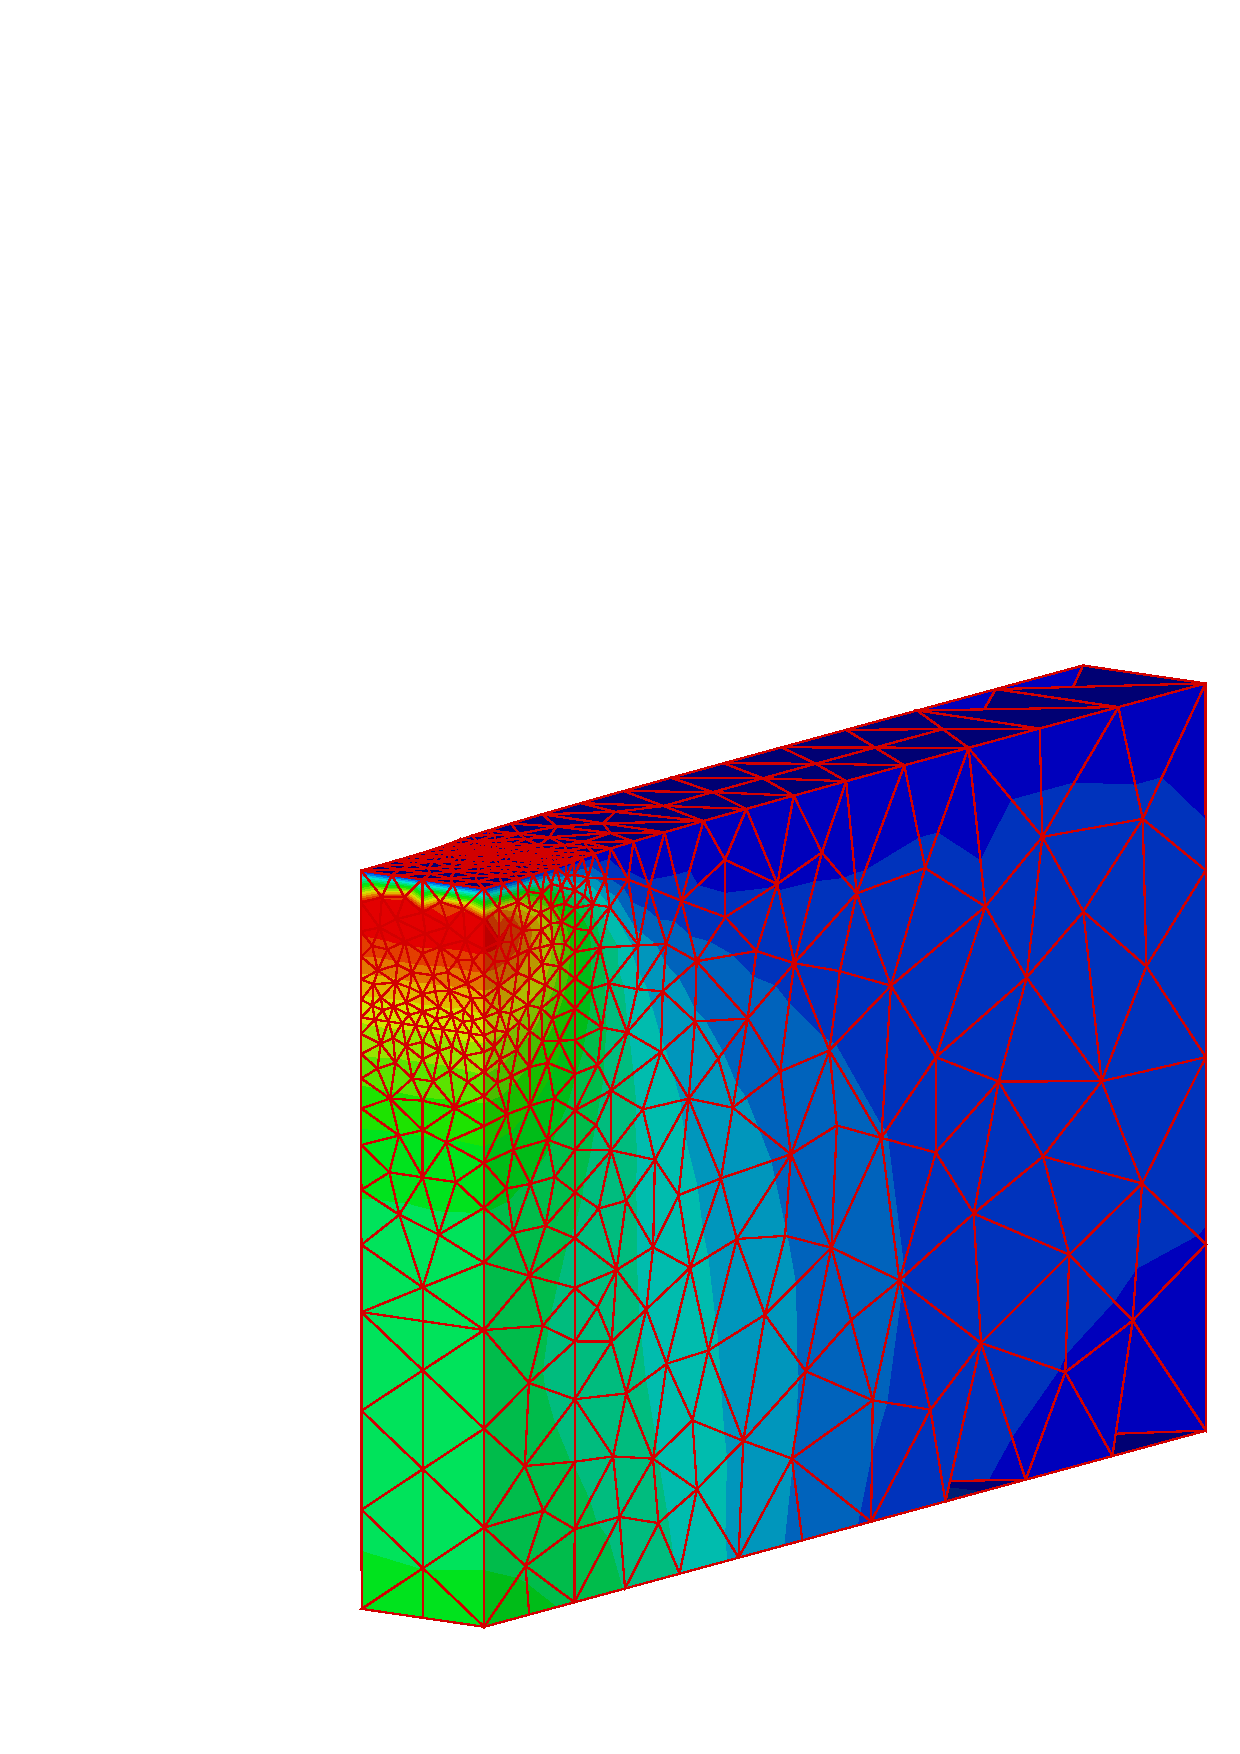
\includegraphics[width=0.44\textwidth]{chapter_14/figures/fig_14_1_4_b}
\end{center}
\vspace{-0.5cm}
\caption{Mesh geometry.}
\label{fig_HM3}
%\vspace{-1.0cm}
\end{figure}

\begin{figure}[!tbh]
\begin{center}
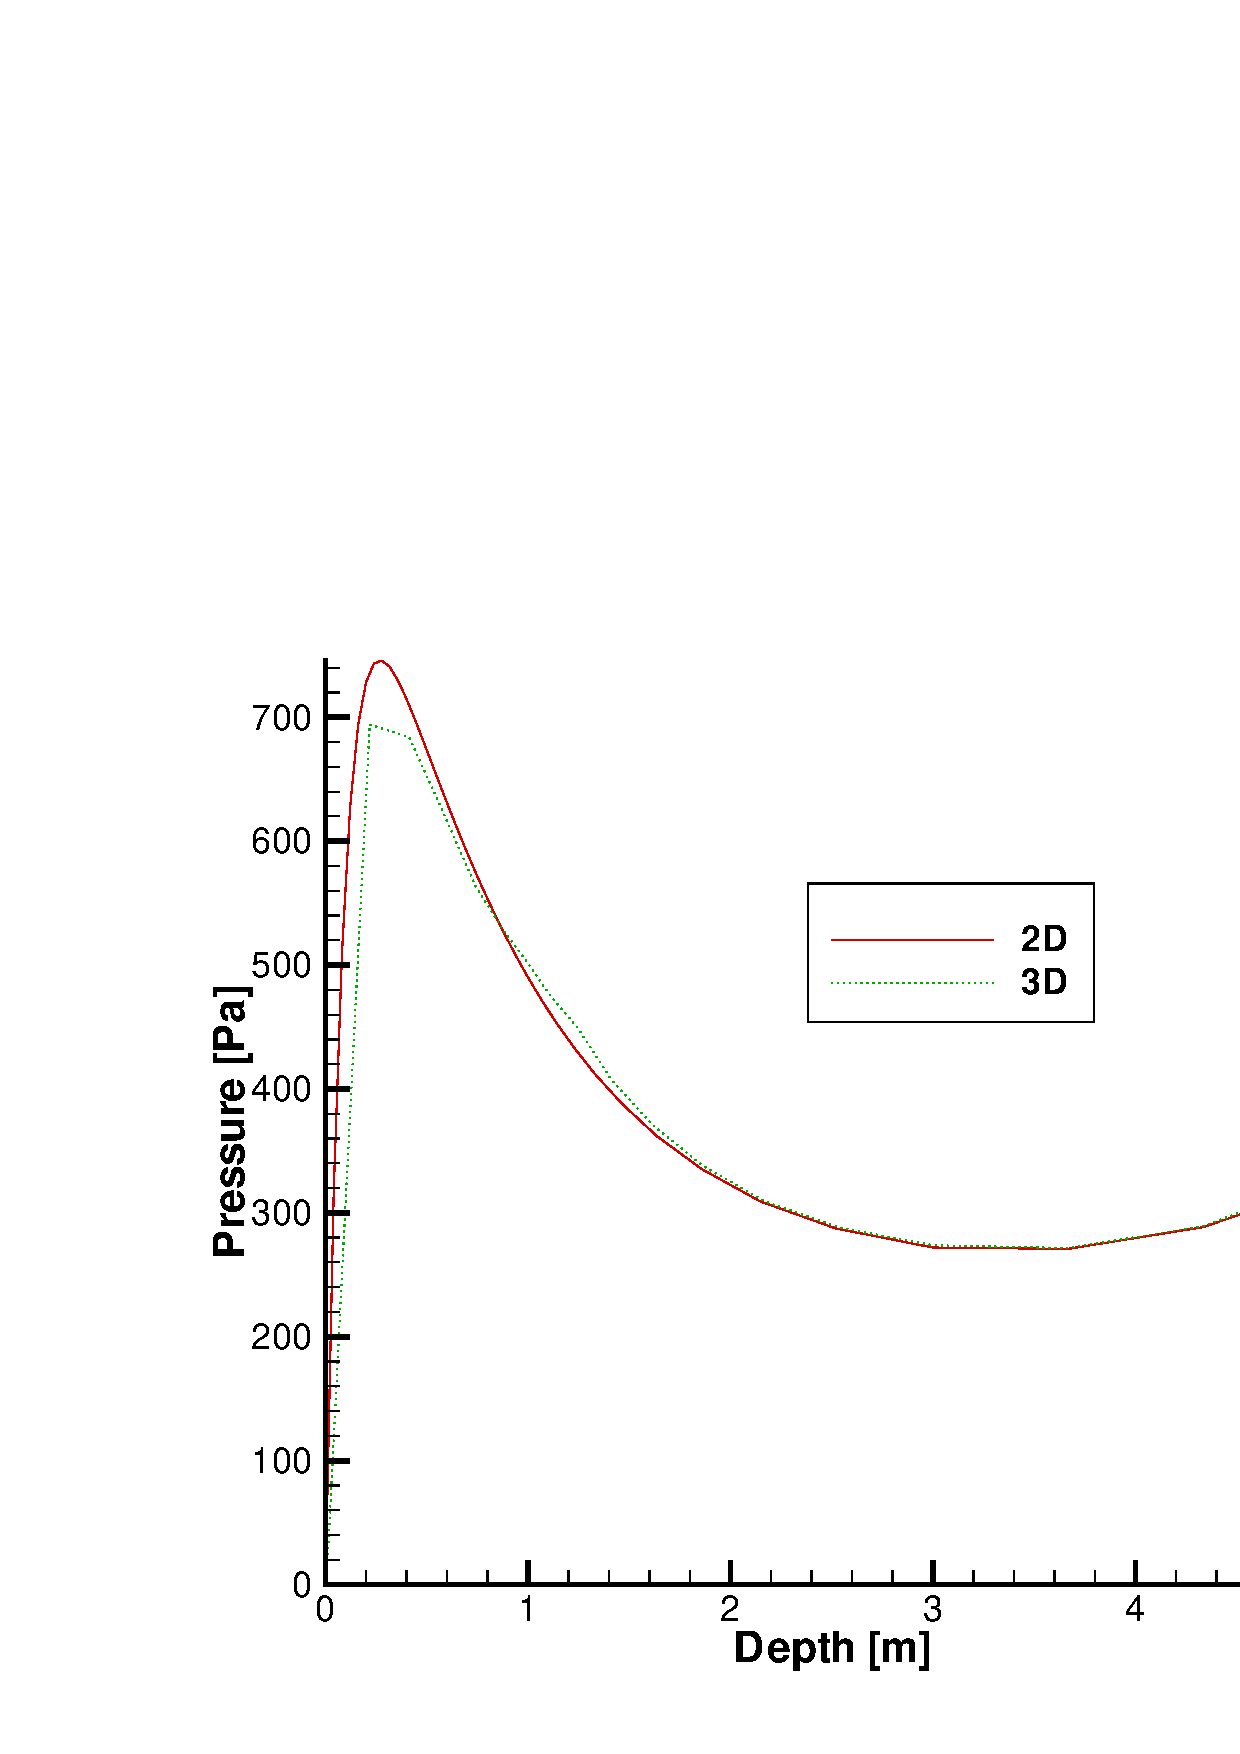
\includegraphics[width=0.49\textwidth]{chapter_14/figures/fig_14_1_5_a}
\includegraphics[width=0.49\textwidth]{chapter_14/figures/fig_14_1_5_b}
\end{center}
\caption{Comparison along symmetric axis.}  
\label{fig:e11}
\end{figure}

\begin{figure}[!tbh]
\begin{center}
\includegraphics[width=0.49\textwidth]{chapter_14/figures/fig_14_1_6_a}
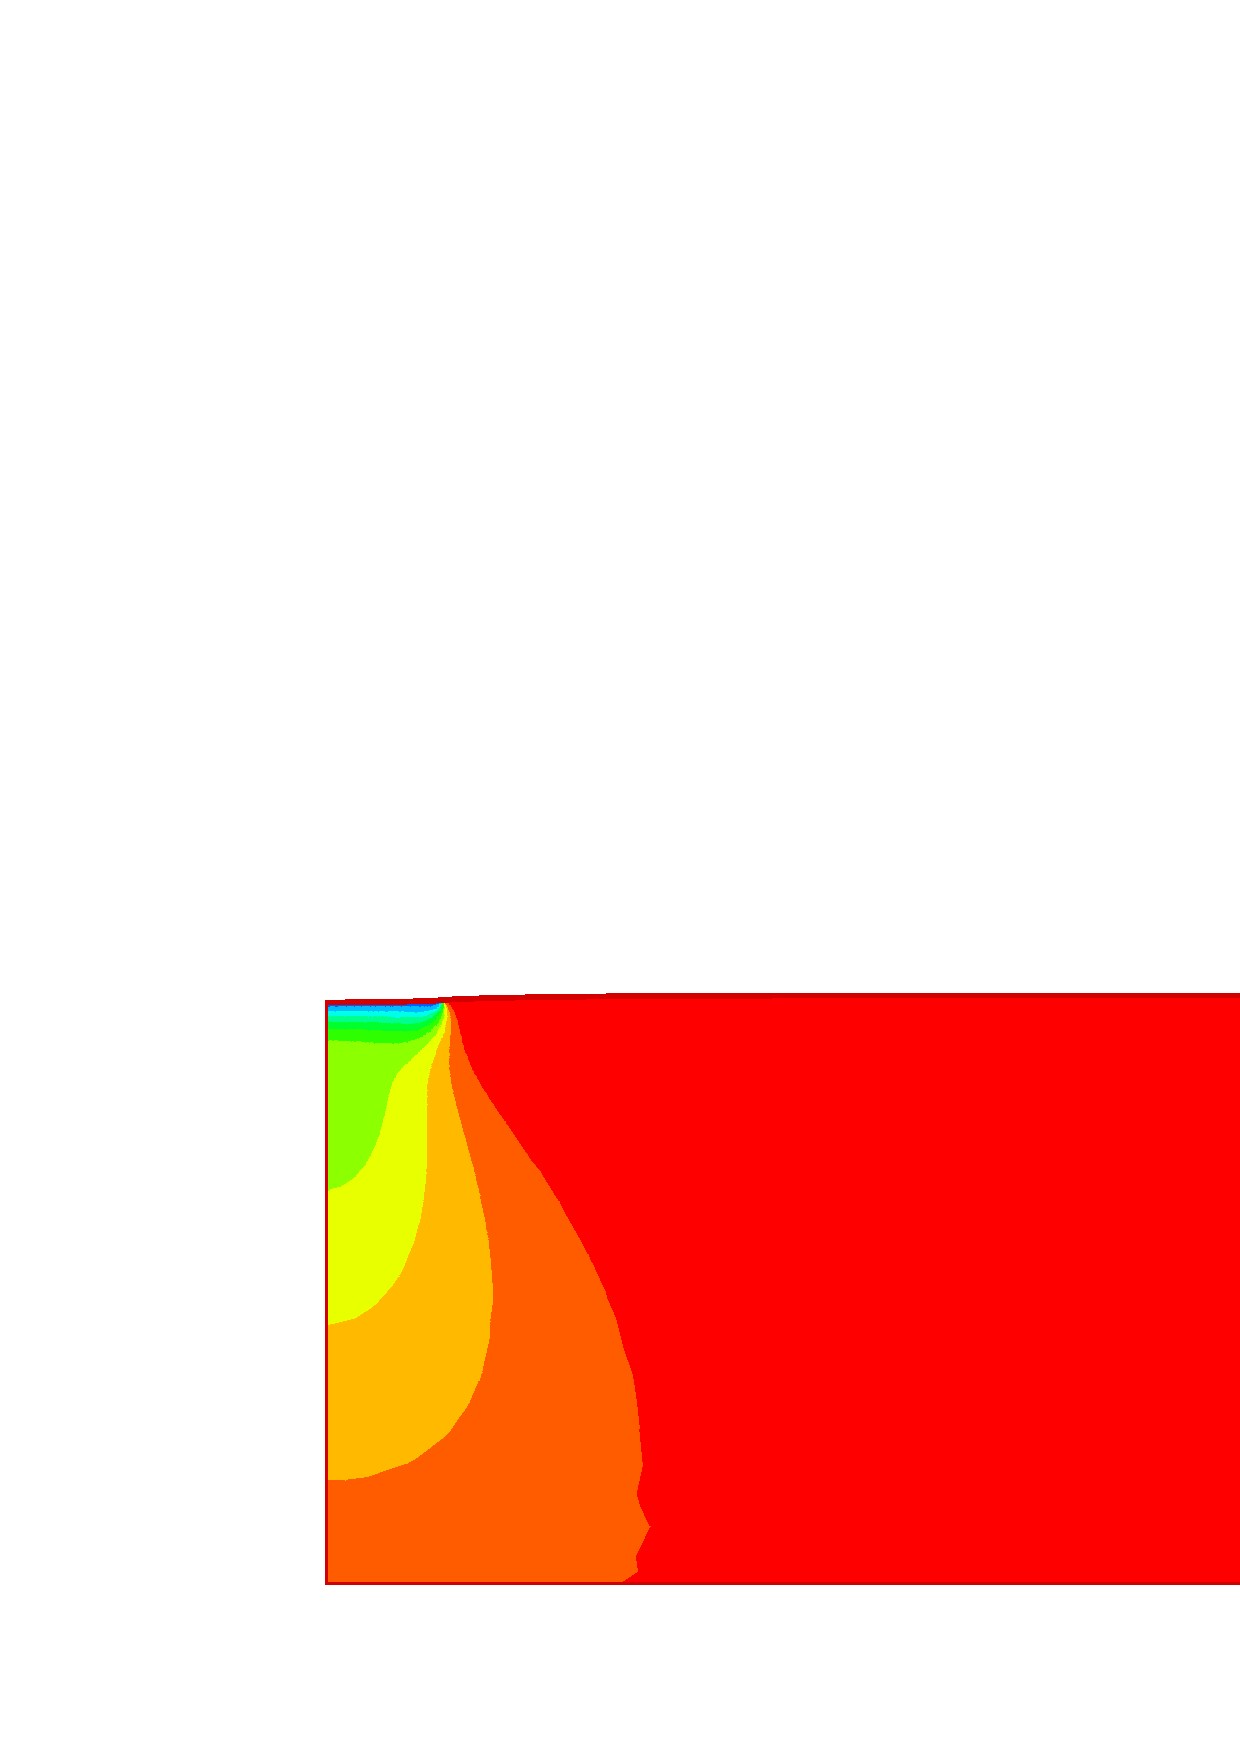
\includegraphics[width=0.49\textwidth]{chapter_14/figures/fig_14_1_6_b}
\end{center}
\vspace{-0.5cm}
\caption{2D contours.}
\label{fig:e10}

\begin{center}
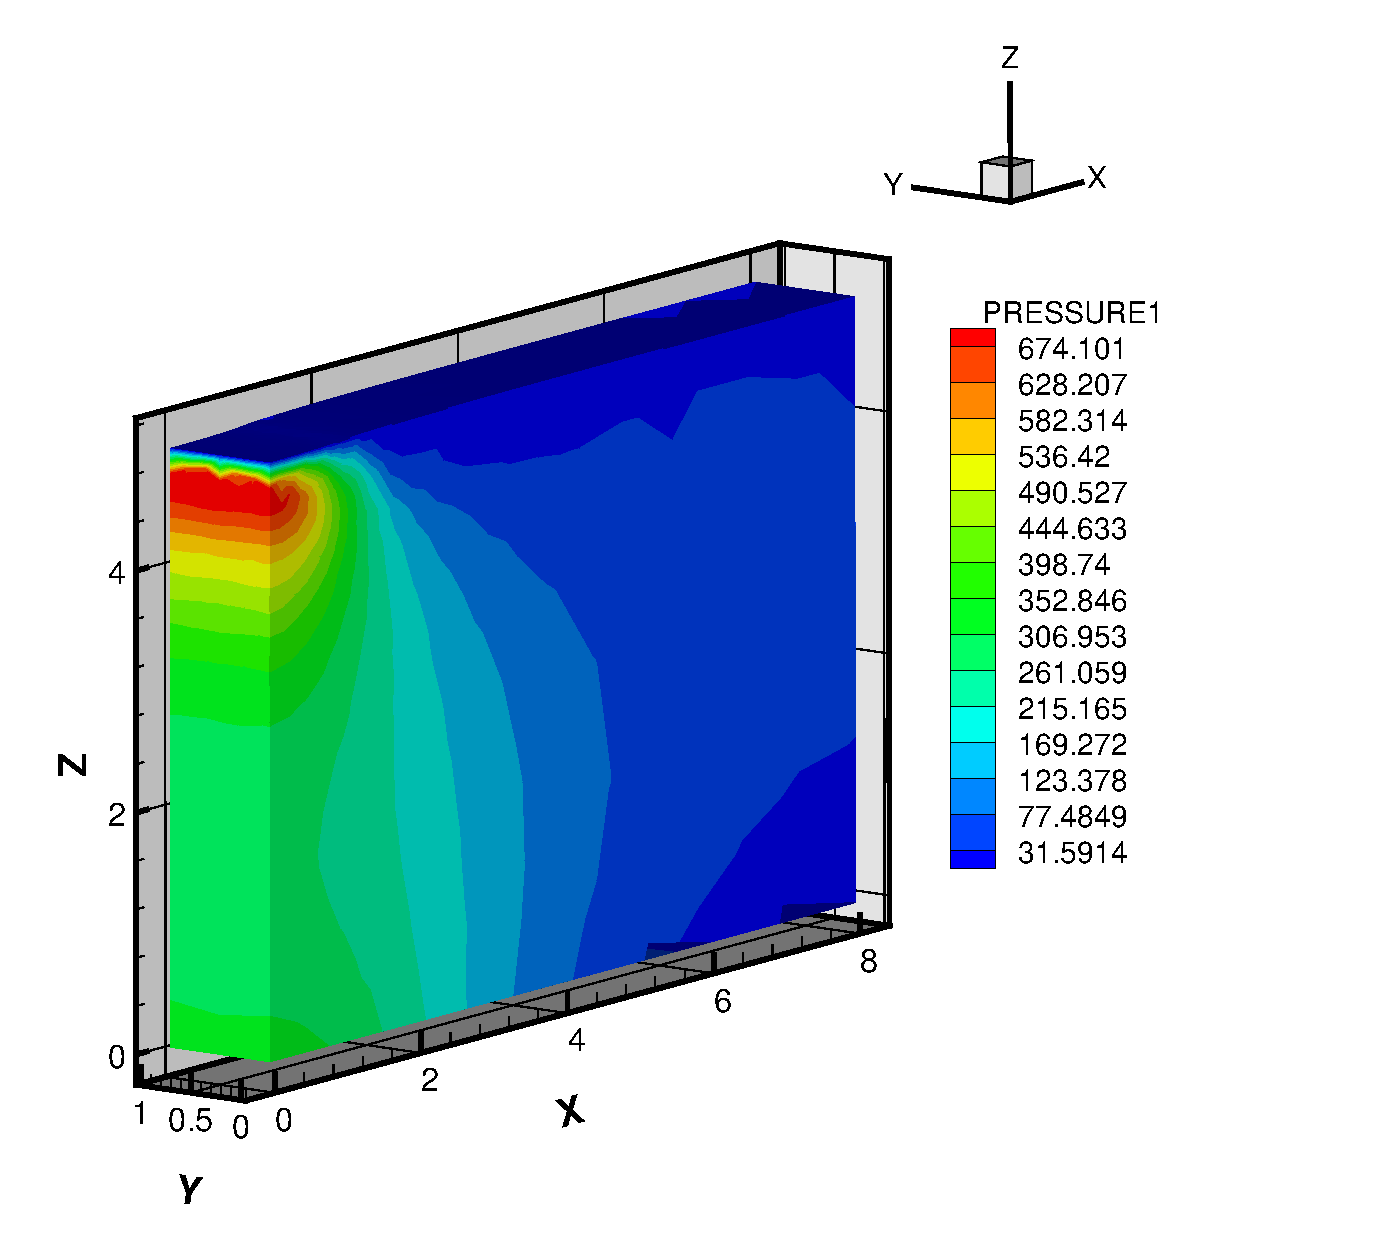
\includegraphics[width=0.49\textwidth]{chapter_14/figures/fig_14_1_7_a}
\includegraphics[width=0.49\textwidth]{chapter_14/figures/fig_14_1_7_b}
\end{center}
\vspace{-0.5cm}
\caption{3D contours.}
\label{fig:e12}
\end{figure}
\subsection{Distributed footing: Poroelastic cube (3D) with dynamic consolidation}
Considering the same problem design as the previous section, the mechanical calculation is now extended to allow for time-dependent deformation. In other words, solid displacements are no longer solved to equilibrium, so that solid velocity may be non-zero following solution of the mechanical system.

\subsubsection*{Definition}
All stresses and pressure are zero at the beginning of deformation. Strip
loading ($\sigma_{yy}=\sigma_0$ in $x\in[0,1]$), zero stresses
($\sigma_{yy}=\sigma_{xy}=0$ in $x\in(1,8]$) and zero pressure at
the top; no horizontal flux, no horizontal displacements and zero
shear stresses at left and right hand sides; no vertical flux and no
displacements at bottom (Figure \ref{fig-setting}).

Material parameters are given in Table \ref{tab:mat-dynam}.

\begin{table}[!htb]
\begin{center}
\begin{tabular}{lll}
\hline{\smallskip}
Property & Value & Unit \\
\hline
Young's modulus & $3\times 10^{4}$  & $N/m^{2}$ \\
Poisson's ratio & $0.2, 0.4$       & $-$ \\
Permeability    & $10^{-10}$        & $m^2$ \\
Fluid viscosity & $10^{-3}$         & $Pa\,s$ \\
\hline
\end{tabular}
\end{center}
\caption{Material properties of dynamic consolidation problem.}
\label{tab:mat-dynam}
\end{table}

\subsubsection*{Results}
Time duration is ten time steps. The following figures, Fig. \ref{fig_dynHM1}--\ref{fig_dynHM4} show the distribution of state variables within the domain after 10 time steps. Such distribution is similar to the static case illustrated in Fig. \ref{fig:e10}.
 
\begin{figure}[!htb]
\begin{center}
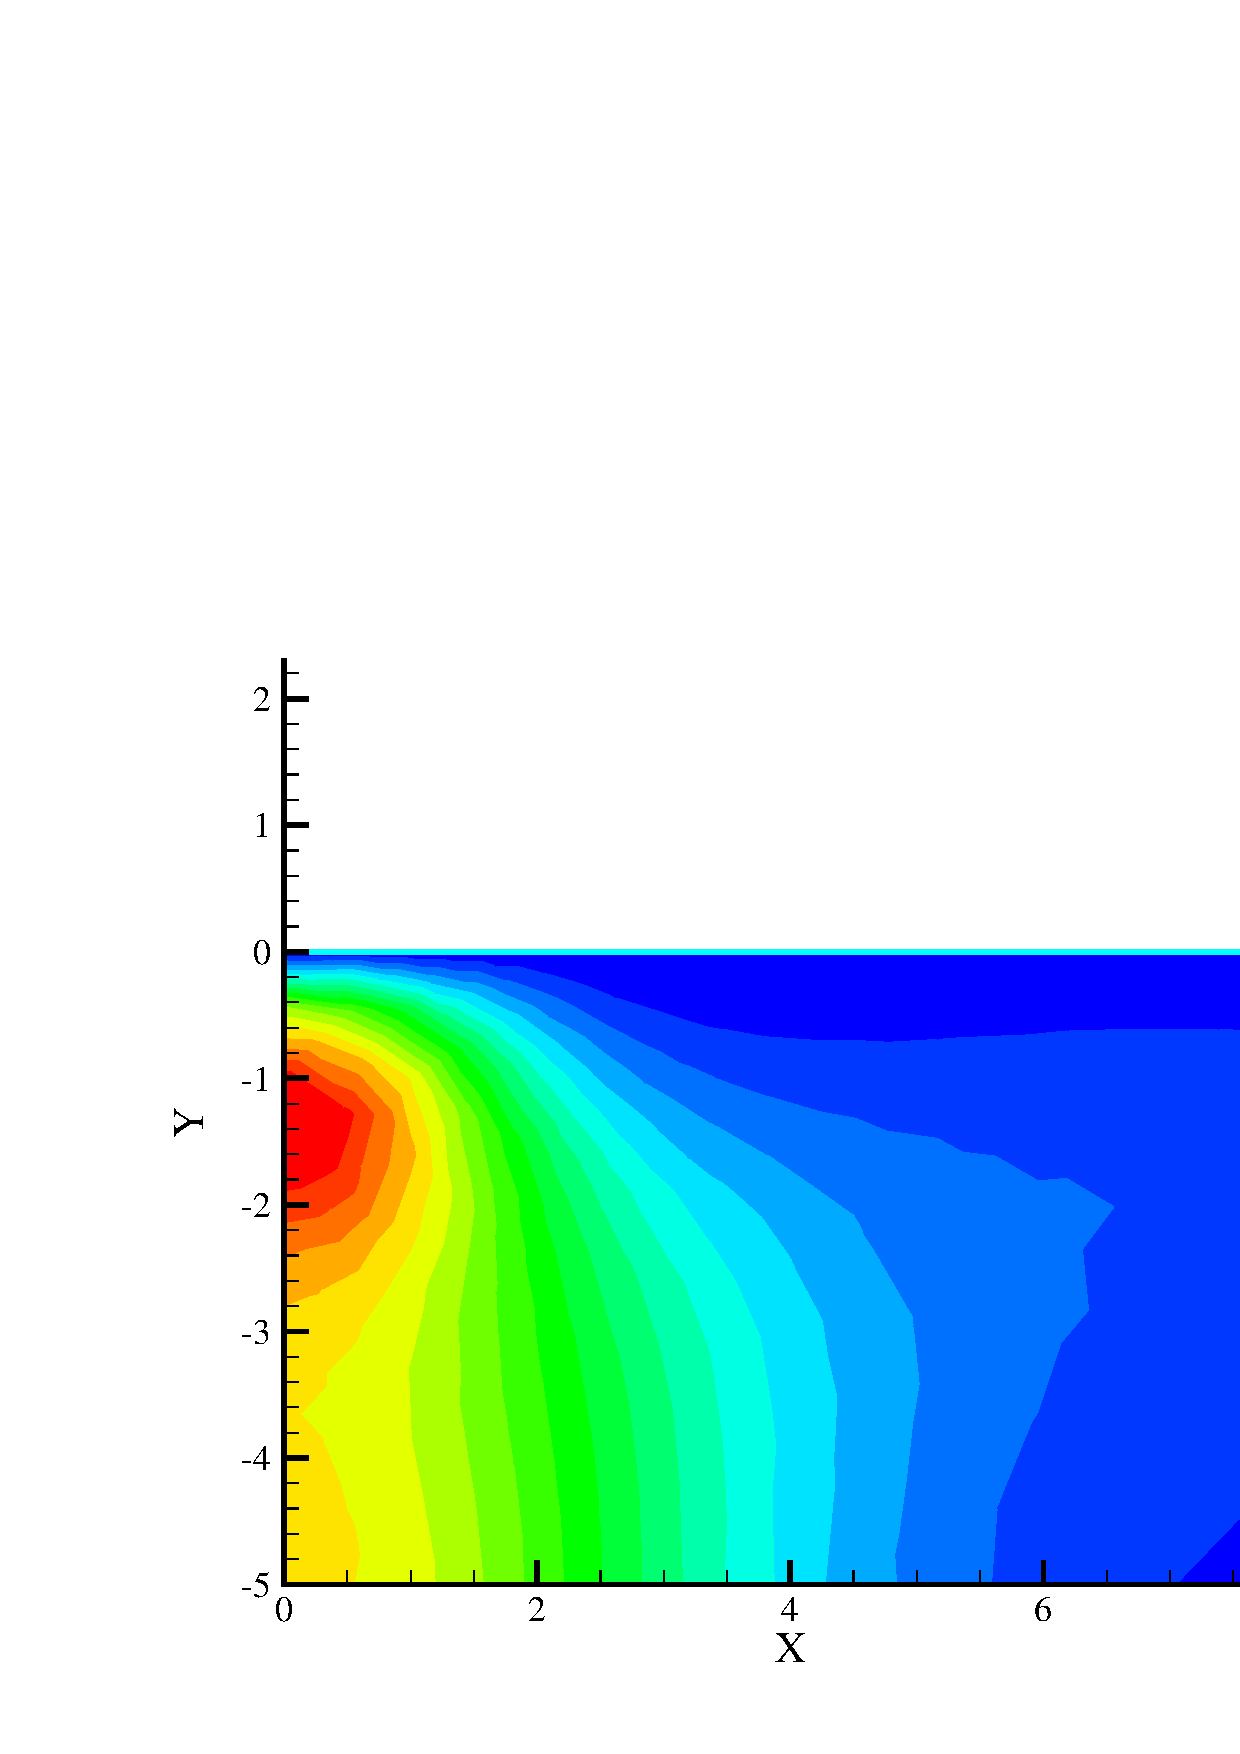
\includegraphics[width=0.49\textwidth]{chapter_14/figures/fig_14_1_8_a}
\includegraphics[width=0.49\textwidth]{chapter_14/figures/fig_14_1_8_b}
\end{center}
\caption{Fluid pressures $p$ and rate of fluid pressure $\dot p$ }
\label{fig_dynHM1}
\end{figure}

\begin{figure}[!htb]
\begin{center}
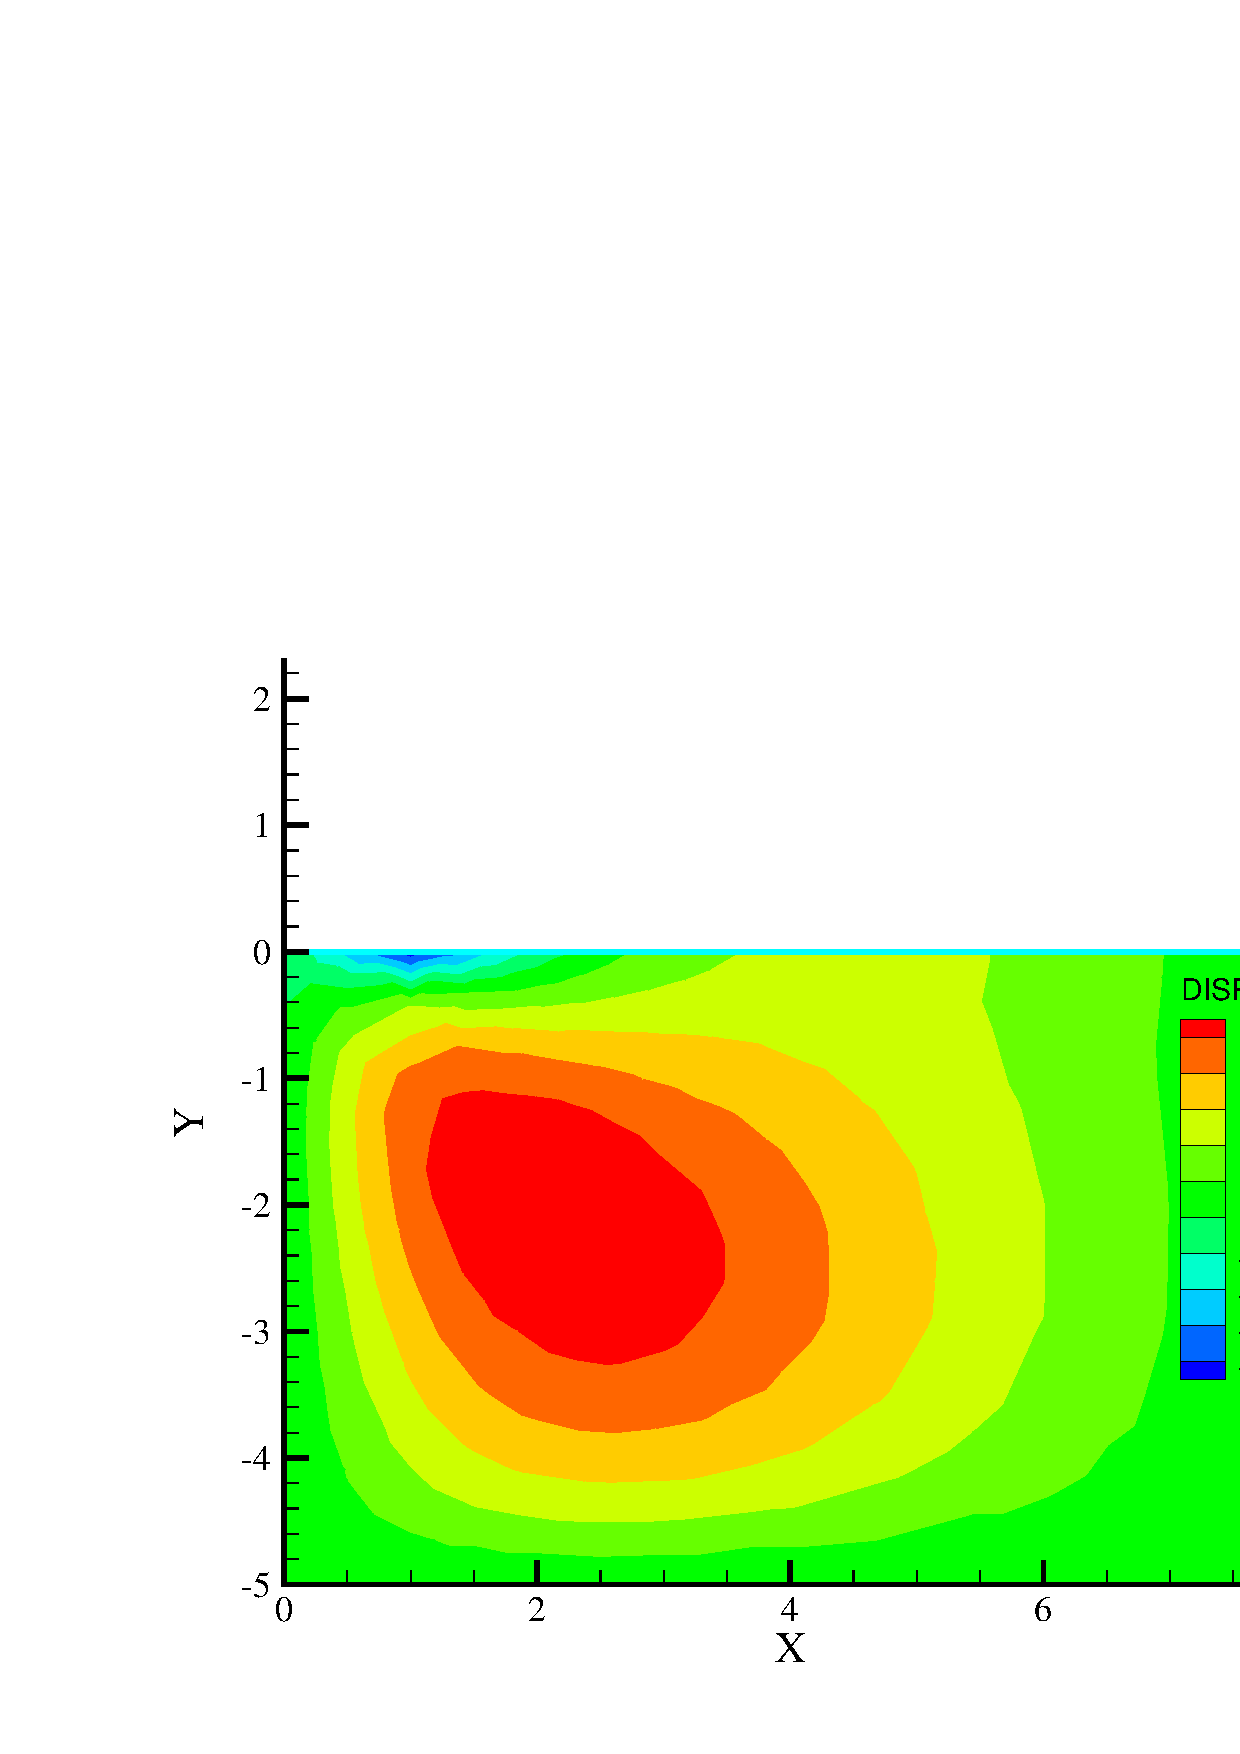
\includegraphics[width=0.32\textwidth]{chapter_14/figures/fig_14_1_9_a}
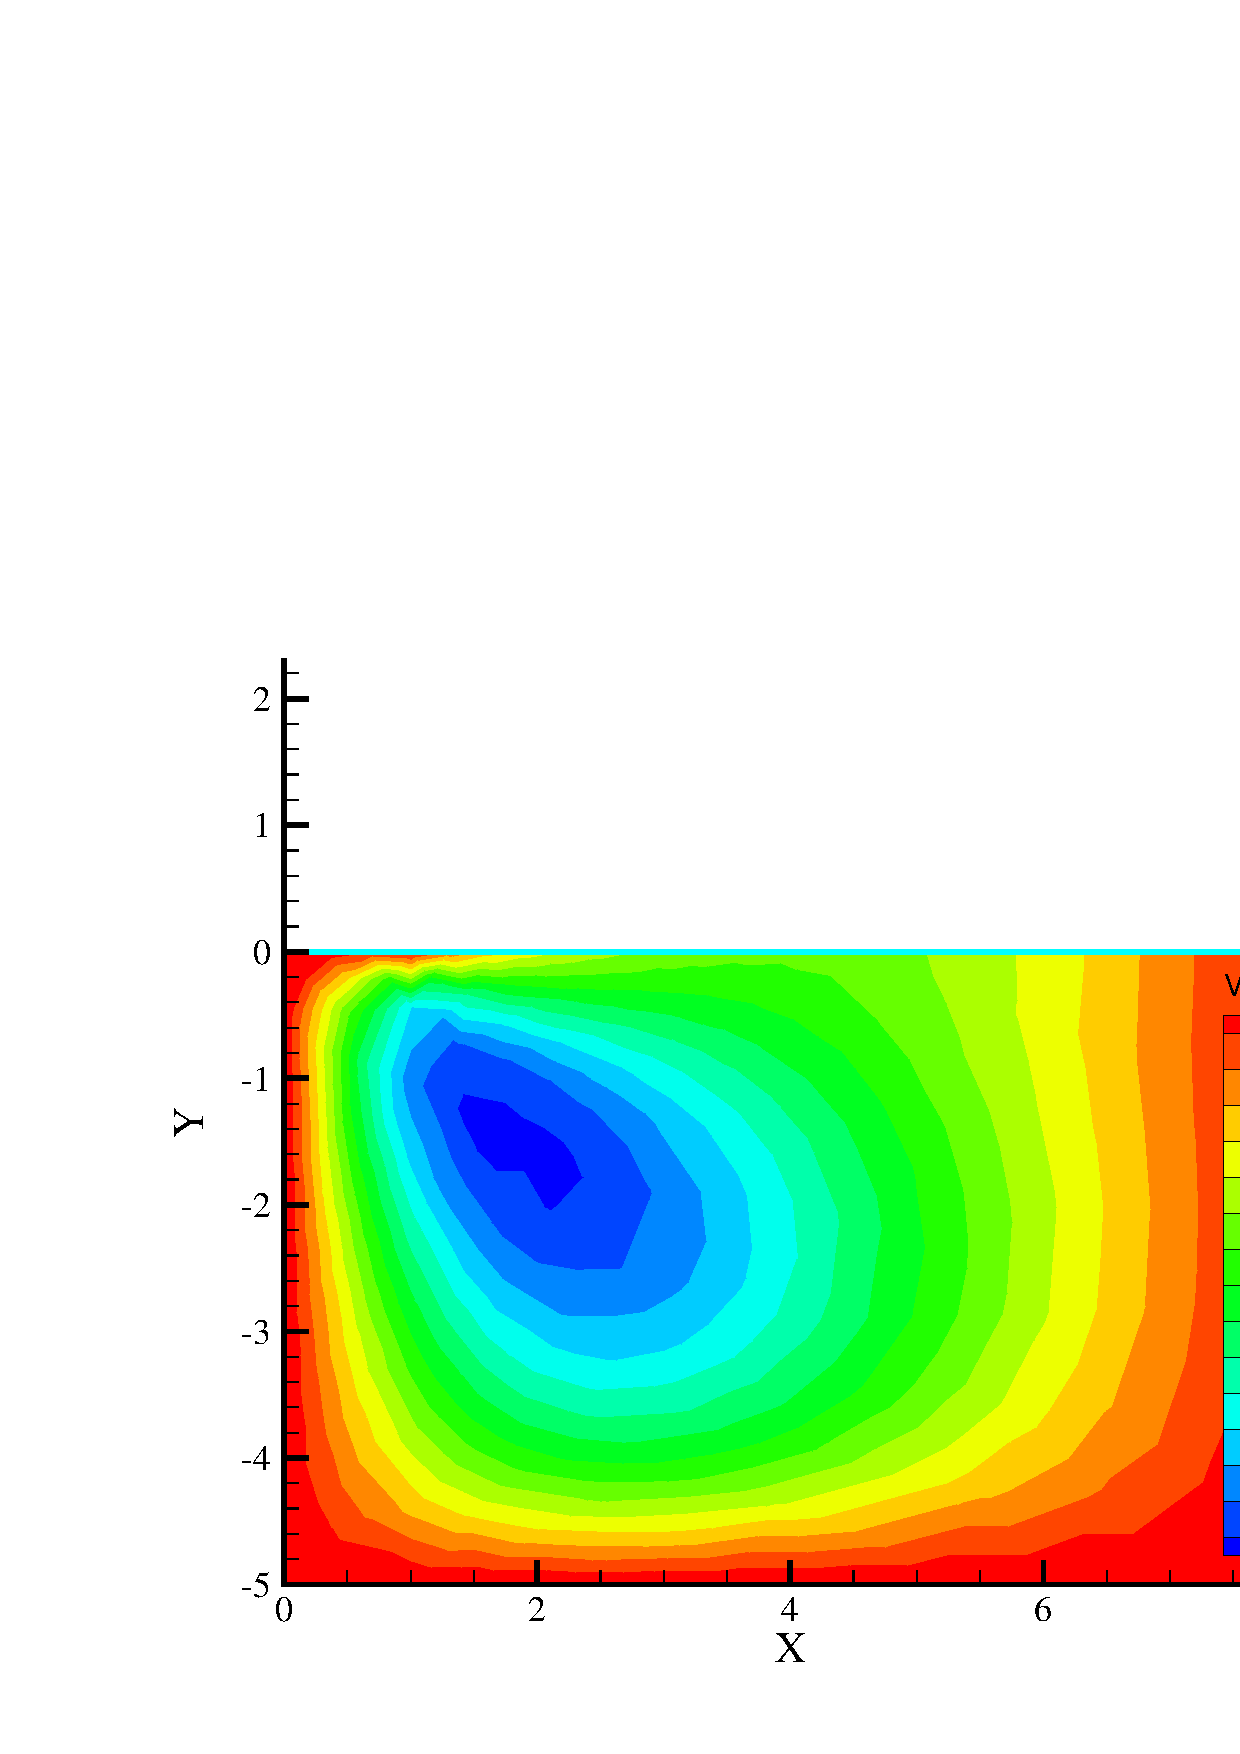
\includegraphics[width=0.32\textwidth]{chapter_14/figures/fig_14_1_9_b}
\includegraphics[width=0.32\textwidth]{chapter_14/figures/fig_14_1_9_c}
\end{center}
\caption{Displacement, its rate and acceleration: horizontal component}
\label{fig_dynHM2}
%\end{figure}
%\begin{figure}[!htb]
\begin{center}
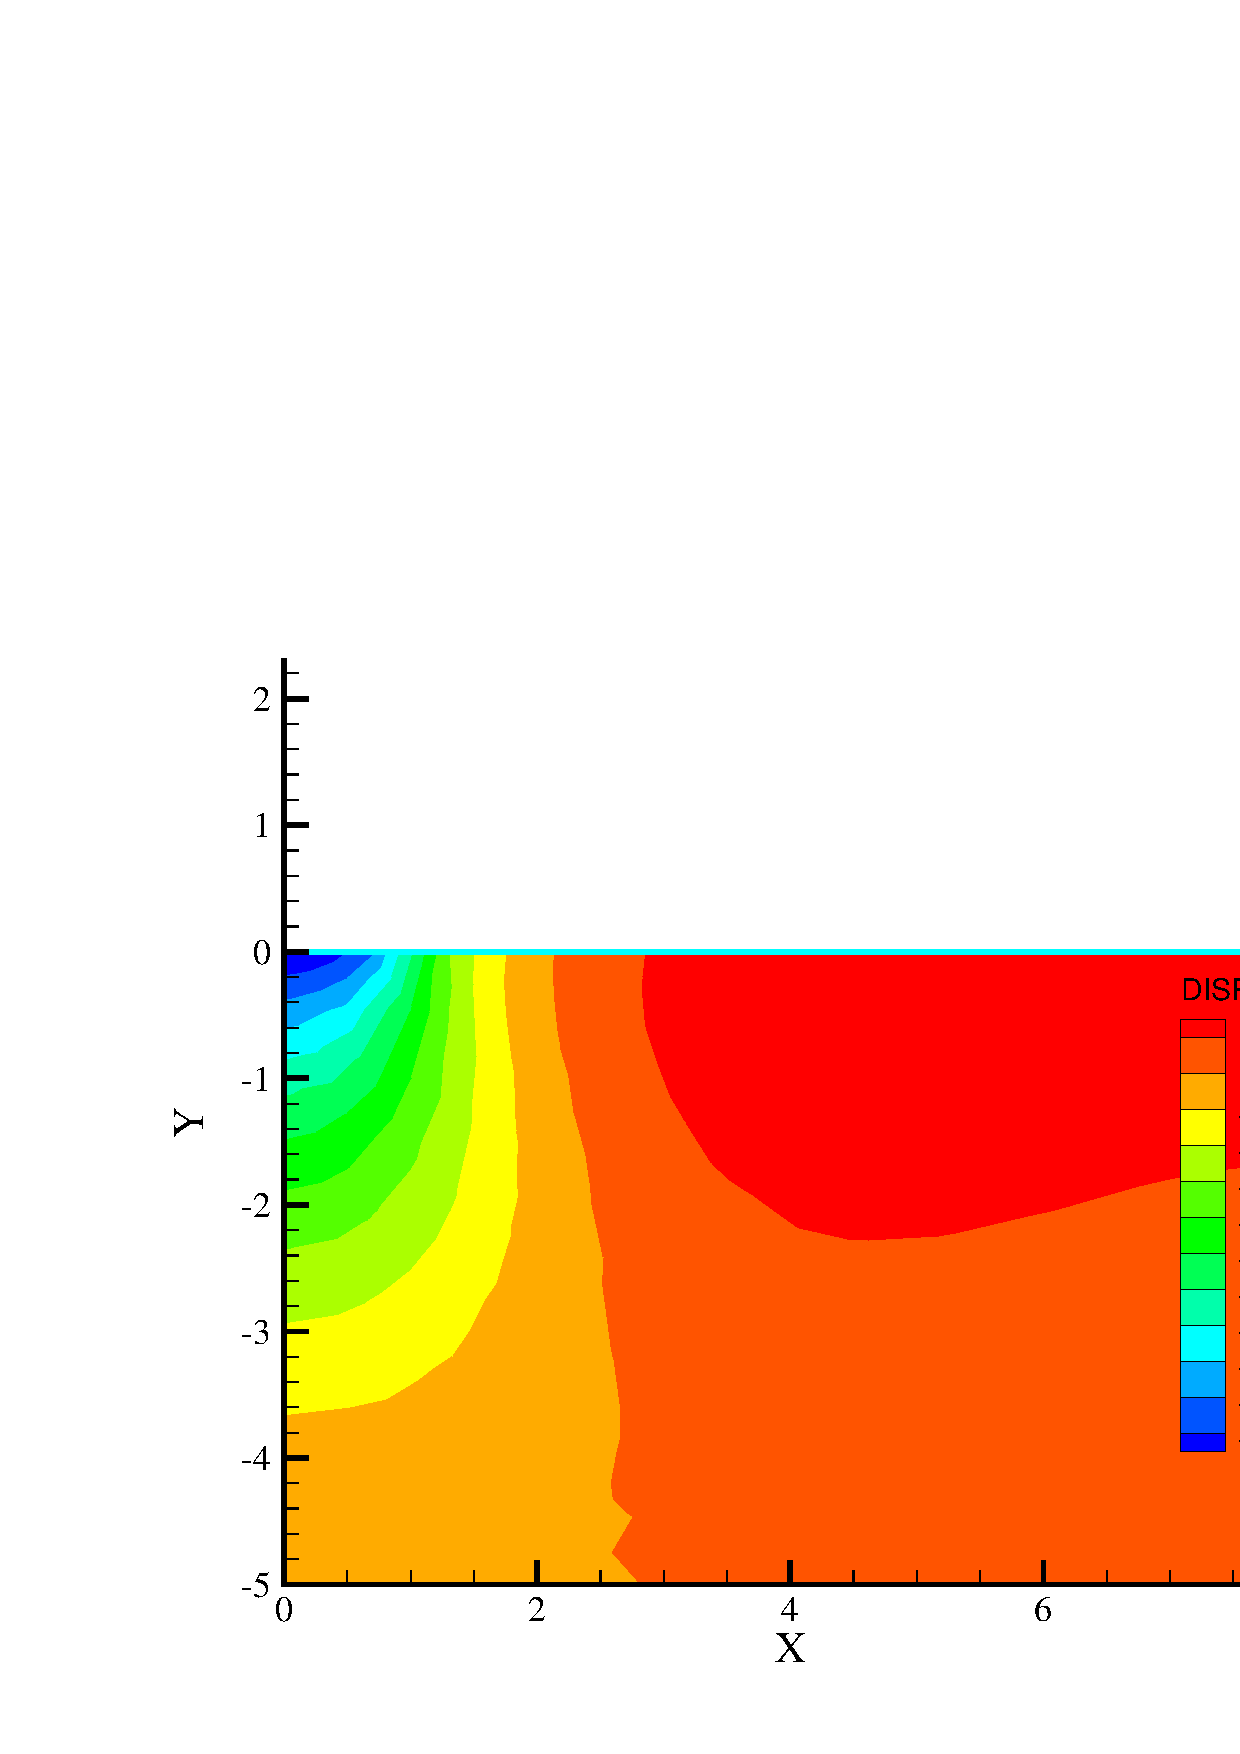
\includegraphics[width=0.32\textwidth]{chapter_14/figures/fig_14_1_10_a}
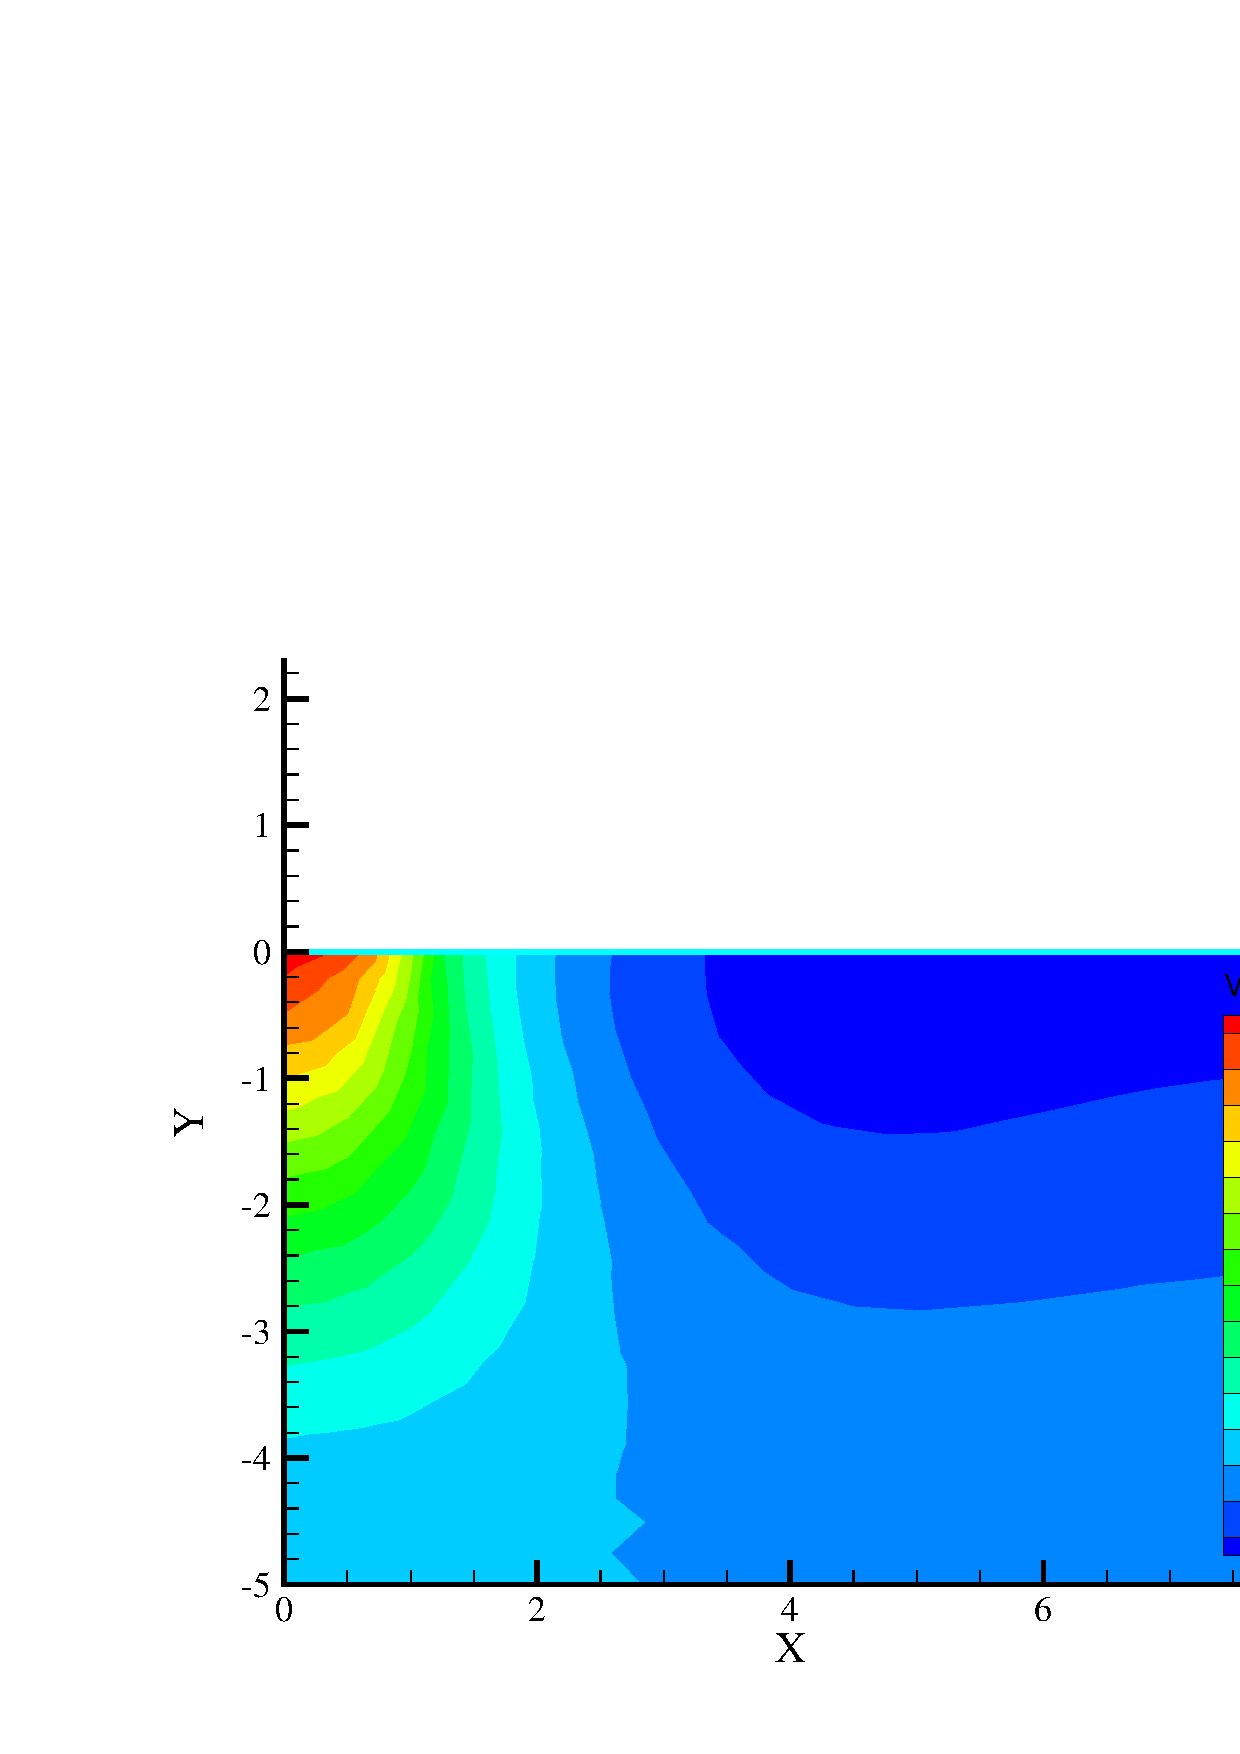
\includegraphics[width=0.32\textwidth]{chapter_14/figures/fig_14_1_10_b}
\includegraphics[width=0.32\textwidth]{chapter_14/figures/fig_14_1_10_c}
\end{center}
\caption{Displacement, its rate and acceleration: vertical component}
\label{fig_dynHM3}
\end{figure}
\begin{figure}[!htb]
\begin{center}
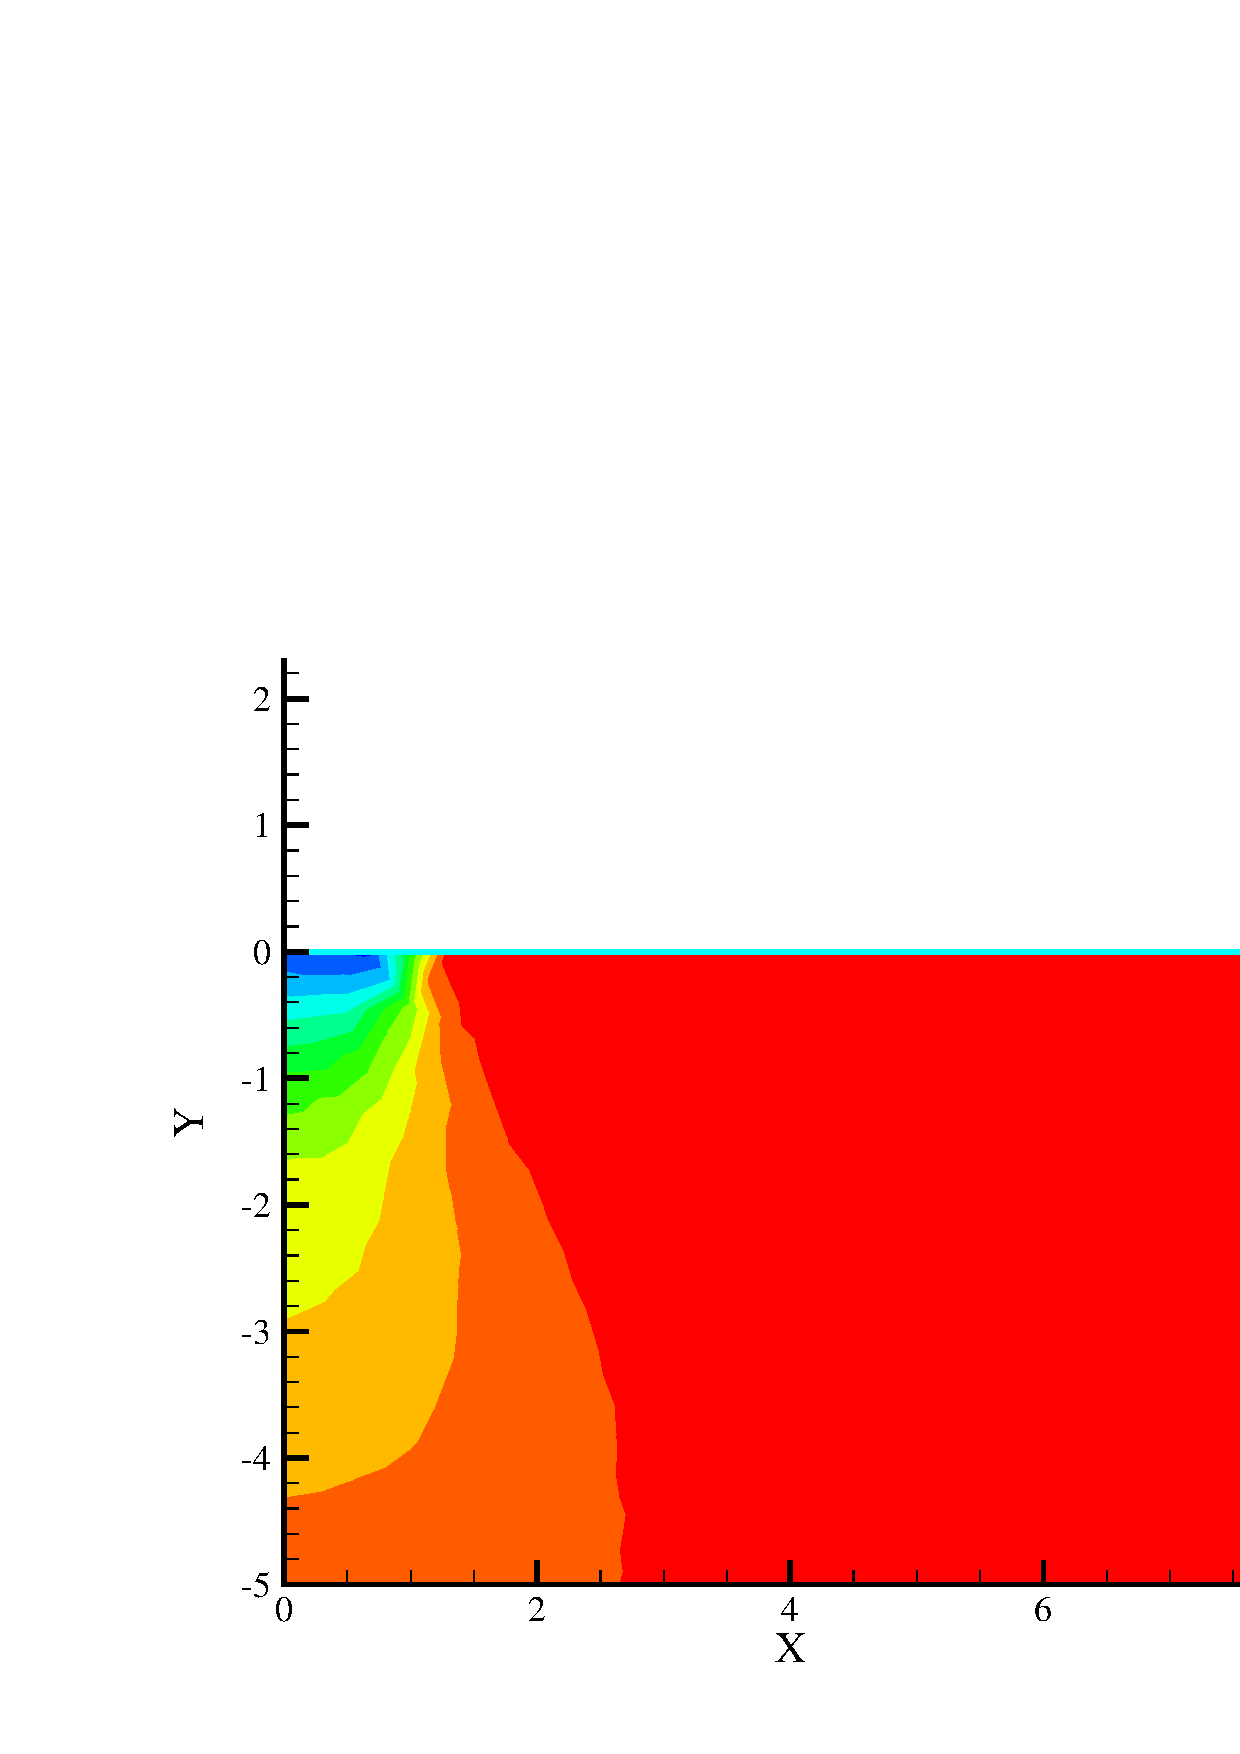
\includegraphics[width=0.5\textwidth]{chapter_14/figures/fig_14_1_11}
\end{center}
\caption{Vertical stress.}
\label{fig_dynHM4}
\end{figure}












